% 11-07.tex
% FDG 2012 conference paper
% WORKS WITH V3.2SP OF ACM_PROC_ARTICLE-SP.CLS
% November 2011
% Author: George Lee, Yongwen Xu, Robert Brewer, Philip Johnson
%
% ----------------------------------------------------------------------------------------------------------------
% This .tex file (and associated .cls V3.2SP) *DOES NOT* produce:
%       1) The Permission Statement
%       2) The Conference (location) Info information
%       3) The Copyright Line with ACM data
%       4) Page numbering
% ---------------------------------------------------------------------------------------------------------------
% It is an example which *does* use the .bib file (from which the .bbl file
% is produced).
% REMEMBER HOWEVER: After having produced the .bbl file,
% and prior to final submission,
% you need to 'insert'  your .bbl file into your source .tex file so as to provide
% ONE 'self-contained' source file.
%

\documentclass{acm_proc_article-sp}

%% Package to linebreak URLs in a sane manner.
\usepackage{url}

\begin{document}

\title{Makahiki: An Open Source Game Engine for Energy Education and Conservation}

%\numberofauthors{1} 

\author{
\smallskip
George E. Lee\\ 
\smallskip
Yongwen Xu\\ 
\smallskip
Robert S. Brewer\\ 
\smallskip
Philip M. Johnson\\
       \affaddr{Information and Computer Sciences}\\
       \affaddr{University of Hawai`i at M\=anoa}\\
       \affaddr{Honolulu, HI 96822}\\
       \email{[gelee, yxu, rbrewer, johnson]@hawaii.edu}
}

\toappear{{\em Submitted to Foundations of Digital Games 2012, Raleigh, North
  Carolina, May 2012.}}

\maketitle
\begin{abstract}
  The rising cost, increasing scarcity, and environmental impact of fossil
  fuels as an energy source makes a transition to cleaner, renewable energy
  sources an international imperative.  This paper presents Makahiki, an open
  source game engine for energy education and conservation. Developed for a
  residence hall energy competition, Makahiki facilitates the implementation of
  ``serious games'' that motivate players to learn about energy issues,
  improve their intuition about energy consumption, and understand how to use energy more
  efficiently in their normal life.  Initial deployment of Makahiki at the
  University of Hawaii in Fall 2011 has revealed useful insights into its game
  mechanics, ways to improve the next Kukui Cup challenge, and insights
  into the changes we need to make to better facilitate adaptation to other energy contexts.
\end{abstract}

% A category with the (minimum) three required fields
\category{L.5.1}{Game-based Learning}{Gaming}

\terms{Human Factors, Games, Education, Motivation}

\keywords{Serious Games, Education, Gamification, Energy}% NOT required for Proceedings

\section{Introduction}

The rising cost, increasing scarcity, and environmental impact of fossil fuels
as an energy source makes a transition to cleaner, renewable energy sources an
international imperative.  One barrier to this transition is the relatively
inexpensive cost of current energy, which makes financial incentives less
effective. Another barrier is the success that electrical utilities have had in
making energy ubiquitous, reliable, and easy to access, thus enabling
widespread ignorance in the general population about basic energy principles
and trade-offs.  In Hawaii, the need for transition is especially acute, as the
state leads the US both in the price of energy (over \$0.30/kWh) and
reliance on fossil fuels as an energy source (over 90\% from oil and coal).

Moving away from petroleum is a technological, political, and social paradigm
shift, requiring citizens to think differently about energy policies, methods
of generation, and their own consumption than they have in the past.
Unfortunately, unlike other civic and community issues, energy has been almost
completely absent from the educational system. To give a sense for this
invisibility, public schools in the United States generally teach about the
structure and importance of our political system (via classes like ``social
studies''), nutrition and health (through ``health''), and even sports (through
``physical education'').  But there is no tradition of teaching ``energy'' as a
core subject area for an educated citizenry, even though energy appears to be
one of the most important emergent issues of the 21st century.

Another emergent issue is the explosive spread of game techniques, not only in
its traditional form of entertainment, but across the entire cultural spectrum.
The adoption of game techniques to non-traditional areas such as finance,
sales, and education has become such a phenomenon that the Gartner Group
included ``gamification'' \cite{Deterding2011mt} on its 2011 Hype List,
positioning it near the summit of ``inflated expectations'' (after which it is
projected to fall into the ``trough of disillusionment'').

This paper describes Makahiki, an open source game engine for energy
conservation and education, in which we attempt to create synergy between
these two emergent issues.  The result of over two years of research and
iterative development, Makahiki explores one section of the design space
where virtual world game mechanics are employed to affect real world energy
behaviors.  The ultimate goal of the Makahiki project is to learn to
not just affect energy behaviors during the course of the game, but to
produce long lasting, sustained change in energy behaviors and
outlooks by participants. 

We used Makahiki to create an energy challenge called The Quest for the Kukui
Cup (hereafter, the Kukui Cup) for approximately 1,000 first year students
living in four residence hall towers at the University of Hawaii in Fall, 2011.
During the three weeks of the competition, over 400 of the eligible students
played the game, for a total of 850 game play hours.  In addition to online
play, the Kukui Cup integrated 24 real world events, including workshops on
energy-related matters, excursions to a wind farm and other energy related
locations, and energy-related activities on campus. The game mechanics were
designed to create a self-reinforcing \emph{virtuous circle} between the real
world and virtual world activities.  The challenge was well received and plans
are already underway to both repeat the challenge in 2012 for University of
Hawaii first year students, and adapt it to other residence halls and other
universities in Hawaii.

The next section briefly reviews the research on which we based Makahiki and
the Kukui Cup. We then discuss the architecture and game mechanics of the
system, followed by the lessons we learned from its first deployment. We
conclude with our goals for improving the system.

\section{Related Work}
Our research draws on work we've done previously
 \cite{csdl2-11-03,csdl2-10-07,csdl2-11-02}, as well as from
work done by others in the areas of energy behavior research, energy 
competitions, gamification and serious games. 

To reduce energy consumption, providing energy feedback is a critical
foundation. Darby's survey of energy consumption studies from the past three
decades found  that consumption in identical homes could differ in energy use
by a factor of two or more depending on the behavior of the inhabitants
\cite{darby-review-2006}. Another survey of energy feedback conducted by
Faruqui et al. found that residents that actively used the in-home displays
with near-realtime feedback averaged a 7\% reduction in energy usage
\cite{Faruqui09}. Darby also points out that feedback alone is not always
enough: other factors such as training could lead to higher rates of energy
conservation \cite{darby-2000-making-it-obvious}.

Energy competitions or challenges have been introduced to college dormitories
and residential homes as ways to facilitate and incentivize energy reduction.
Petersen et al. describe their experiences deploying a real-time feedback
system in an Oberlin College dorm energy competition in 2005 that includes 22
dormitories over a 2-week period \cite{petersen-dorm-energy-reduction}. Web
pages were used to provide feedback to students. They found a 32\% reduction in
electricity use across all dormitories. However, in a post-competition survey,
respondents indicated that some behaviors, such as turning off hallway lights
at night and unplugging vending machines were not sustainable outside the
competition period.  Overall, there has been little analysis on energy usage
after competitions finish, or how positive behavior changes could be sustained.

The Building Dashboard \cite{building-dashboard}, developed by Lucid Design 
Group, is used to support Oberlin's dorm energy competition,
as well as the Campus Conservation Nationals, a nationwide electricity and 
water use reduction competition on college campuses \cite{competetoreduce}. 
The Building Dashboard enables viewing, comparing and sharing building energy
and water use information on the web in compelling visual interface, but the 
cost of the system creates the barrier for wider adoptions. In addition, the 
building dashboard solutions focus on providing energy information as 
a passive media. There is little interaction between participants and the system.

Games on the other hand, have been shown with great potential as successful
interactive media that provide engaging interfaces in various serious contexts
\cite{mcgonigal2011reality,reeves2009total}. Priebatsch attempts to build a
game layer on top of the world with his location-based service startup
\cite{Priebatsch2010ted}.

Reeves et al. described the design of Power House, an energy game that connects
home smart meters to an online multiple player game with the goal to improve
home energy behavior \cite{Reeves2011powerhouse}. In the game, the real world
energy data are transformed into a ``more palatable and relevant form of
feedback'', and players may be incentivized by the in-game rewards to complete
more energy-friendly real-world behaviors.

ROI Research and Recyclebank launched the Green Your Home Challenge as a case 
study of employing gamification techniques online to 
encourage residential green behavioral changes offline \cite{gamingforgood}. 
Working with Google Analytics, the results show a 71\% increase in unique 
visitors and 97\% of participants surveyed said that the challenge increased 
their knowledge about how to help the environment. 

Blending of real and virtual worlds has been explored in broader contexts.
McGonigal designed the award winning serious Alternative Reality Game (ARG)
``World Without Oil'' \cite{worldwithoutoil} and later ``Evoke''
\cite{urgentevoke} with the goal to empower people to come up with creative
solutions to our most urgent real-world problems. ARGs have also been used to
support learning. Connolly et al. discuss the development of an educational ARG
to motivate secondary school students across Europe to learn foreign languages
\cite{connolly2009arguing}. The results of the pilot run of the game in 2009
indicated that 92\% of students felt the game motivated students to learn a
second language. One of problems the team identified is the limitation of
Moodle platform the game is based on.

The report of the ARGOSI project provides insights to the use of ARGs in game
based learning and the challenges in the field of higher education
\cite{whitton2009alternate}. The pilot was run at the University of Bolton with 
the aim to provide an engaging alternative to traditional methods of 
introducing students to university life. The overall up-take of the game was 
fairly low with 173 players and 23 (13\%) of whom were active. The project
identifies a number of questions surrounding educational ARGs, such as 
motivation, relationship to curriculum, marketing and timing. The report 
suggests that a complete ARG model may not be appropriate for wholesale
learning, but there is certainly potential in using game elements.

\section{System Design}
\begin{figure*}[t!]
  \center
  \includegraphics[width=0.4\textwidth, angle=90]{makahiki-architecture.eps}
  \caption{\em \small Architecture of Makahiki}
  \label{fig:MakahikiArchitecture}
\end{figure*}

Section \ref{sys:competition} describes the design of the competition itself. Section \ref{sys:Architecture} discusses the underlying technology of Makahiki and the 2011 Kukui Cup, while section \ref{sys:GameDesign} details the various games and game elements we implemented for the competition.

\subsection{Competition Design}
\label{sys:competition}

The 2011 Kukui Cup took place in four residence hall towers, each containing 10 floors of residents with a total over 250 first-year students. Smart meters were installed on each residential floor of the towers, but due to the electrical infrastructure, energy use could only be tracked by pairs of floors. These pairs of floors share a common lounge space and elevator, so the pairs are called ``lounges''. The lounges across all four towers competed to minimize energy use during the competition, measured in kilowatt-hours.

In addition to the energy competition, there was also a point competition. Each player earned points by performing certain activities through our web application, such as watching a short video about energy (followed by a question), attending events, and making public commitments to adopt more sustainable behaviors. Points were also aggregated to provide lounge-level performance.

\subsection{Architecture}
\label{sys:Architecture}

Figure \ref{fig:MakahikiArchitecture} provides an overview of the different components of Makahiki and how they interoperate. The web application component of Makahiki is implemented using the Django web framework in the Python programming language. In addition to the modules we created, we used other third party libraries including ``django\_cas'' (an authentication plugin that allows players to authenticate using a Common Authentication Service server), ``brabeion'' (a Django module for badges), ``minidetector'' (detects if a client is a mobile phone), and ``restclient'' (a library for interacting with RESTful web services). The website is hosted on a Xserve running Mac OS X 10.6 and Apache. To handle server loads more efficiently, we used memcached (an in-memory caching system) to cache parts of the website for quicker access.

The energy data are handled by another system we developed called WattDepot 
\cite{csdl2-10-05}. WattDepot retrieves energy data from the individual smart meters in the residence halls, and provides that data to clients via a REST API. However, providing particular energy values can be computationally expensive if we have to calculate it every time a player accesses a page. To reduce this computational overhead, we implemented a ``cloud cache'' that uses Google Spreadsheets to store precomputed energy values for the different lounges in the competition. The player's browser accesses the public spreadsheet using client-side Javascript and the Google GData library. The server may access the cloud cache or WattDepot directly, depending on its needs. For example, to award points in the energy goal game (see Section \ref{sys:goal-game}), a script is executed on the server once a day to check the daily energy goal spreadsheet and see if the individual lounges made their goal. Energy data for the lounges over the past 30 days are also stored in a spreadsheet, so we can use client-side Javascript to compute the energy used during the competition.

\subsection{Game Design}
\label{sys:GameDesign}

While developing Makahiki, we constructed several components and games for players to keep them more engaged. The following sections will discuss how each of these components and games contribute to the overall system.

\subsubsection{Rounds}

As part of the configuration for Makahiki, a competition period can be split up into rounds. The energy usage and points during a round are tracked separately but still contribute to the overall totals. If there is no round configured during the competition period, then the overall score is tracked. As an example, the 2011 Kukui Cup was three weeks and had two week long rounds (Round 3 was the overall round). This configuration had the interesting side effect of putting the top players in Round 1 at a disadvantage during Round 2, since they have completed most of the tasks available to them. Players who were new to the competition in Round 2 could complete tasks that were available in Round 1, although they did miss out on any events and excursions that happened during that time.

\begin{figure}[ht!]
  \center
  \includegraphics[width=0.4\textwidth]{smart-grid.eps}
  \caption{\em \small Smart Grid Game}
  \label{fig:SmartGrid}
\end{figure}

\subsubsection{Smart Grid Game}

One of the primary components of Makahiki is the Smart Grid Game shown in Figure \ref{fig:SmartGrid}. This grid is the primary place players go to to earn points in the competition. Tasks are organized into a grid of squares (hence the name ``Smart Grid'') and organized by category columns. The grid contains four different types of tasks: activities, commitments, events, and excursions.

Activities are the most basic task available in the Smart Grid. In order to get points for an activity, a player will have to provide a response to the administrators. These responses can be a short textual answer or an uploaded picture. Administrators access a special admin section of the web application to approve or deny submissions. If a submission is approved, the player will receive the points for their submission. Otherwise, a player will be sent a website notification informing them that their submission was not approved, and a textual description by an administrator of why it was rejected. The player can change and resubmit their response and still earn the full point value for that task.

Commitments are pledges that the player will do something sustainable for a period of five days. Examples include: reducing shower time, taking the stairs, and turning off the lights when leaving a room. Because these commitments are not verifiable, they are worth fewer points than activities. Furthermore, a player can only have up to five active commitments at any given time. After the five day period is up, the player can then declare that they completed the commitment and immediately earn their points. They can then sign up for another commitment, including the one they just completed.

Events and excursions are tied to real world activities. Events are held on campus while excursions take place off campus. Seating is limited, so players are asked to sign up for events they wish to attend. Players that do so are provided with a 2 point signup bonus. Players can also set up a reminder that is sent to their email and/or their mobile phone before the event takes place. At the event, an administrator will hand out attendance codes printed on slips of paper that can be entered on the website. These attendance codes are generated by Makahiki and can only be used once. To discourage players from signing up and not attending, a 2 point penalty is assessed to players who do not submit an attendance code. If the player submits an attendance code for the event after receiving this penalty, the penalty is reversed.

Not all of the tasks in the Smart Grid Game are necessarily available at
the start of the game. We implemented a set of predicates that can be used to determine if a task is locked or unlocked for a player. These predicates include: completed a certain number of tasks within a category, completed all tasks within a category, completed certain tasks, and time-based unlocking (available after a certain date).

These predicates are implemented using a limited subset of Python and can
be changed within the Django admin interface. Competition designers can use
logical operators to combine any of these functions in order to organize
the players' path through the Smart Grid Game.

\subsubsection{Daily Energy Goal Game}
\label{sys:goal-game}

Players are also provided with a daily energy goal. The goal for each lounge is typically a percent reduction from their baseline usage before the competition and is stored in a Google Spreadsheet. When a player goes to the energy page of the web application, they can view their lounge's current progress toward their daily energy goal. Near the end of the day, Makahiki checks the spreadsheet to see if a floor reached their goal. If the floor did reach their goal, each member of the floor that is participating in the game receives 20 points. The energy goal game provides a link between the energy conservation competition and the point competition.

\begin{figure}[t!]
  \center
  \includegraphics[width=0.4\textwidth]{daily-energy-goal-game.eps}
  \caption{\em \small Daily Energy Goal Game visualization}
  \label{fig:DailyEnergyGoal}
\end{figure}

Figure \ref{fig:DailyEnergyGoal} shows what a player would see when they go to the energy page. The Daily Energy Goal display shows both their current progress and their goal so far for two reasons. First, everyone will be under their actual energy goal for most of the day, so this display would not be very useful. Second, we have noticed that the students in the residence halls use more energy at night rather than during the day. Thus, it is easy to be under for most of the day and then jump over the goal at the very end. Displaying their goal so far provides a pace for players to follow. 

\subsubsection{Raffle Game}

\begin{figure}[t!]
  \center
  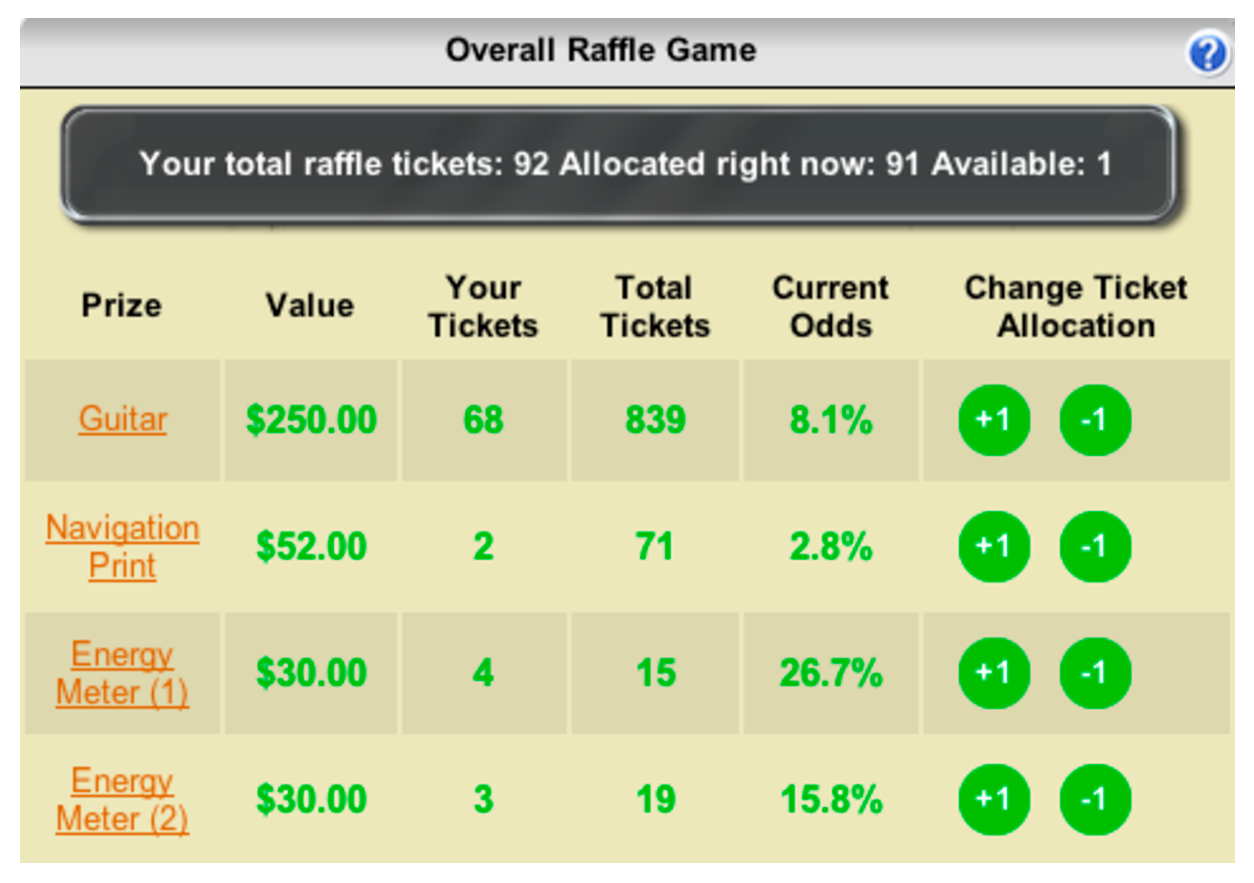
\includegraphics[width=0.4\textwidth]{raffle-small.eps}
  \caption{\em \small Raffle Game for the Overall Round}
  \label{fig:RaffleGame}
\end{figure}

In addition to the prizes awarded to individuals and lounges for earning the most points and conserving the most energy, players can also earn prizes through the Raffle Game. For every 25 points a player earns, they receive one virtual raffle ticket. Players can dynamically allocate their tickets to any raffle prizes they are interested in at any time, up to the end of the raffle. Each round of the competition has its own set of raffle prizes and any unused raffle tickets carry over to the next round. Raffle tickets are independent from a player's score; allocating a raffle ticket does not affect their rank. Figure \ref{fig:RaffleGame} shows an example of the Raffle Game based on the last round of the 2011 Kukui Cup.

\subsubsection{Social and Referral Bonuses}

In an effort to get more people to participate in the competition, we implemented two types of bonuses; social and referral. The social bonus is an administrator option when a task is created in the Smart Grid Game. It awards extra points if the player has done the task with someone else. Examples of tasks with social bonus include attending an event, recording a song related to energy, or measuring a shower water flow rate. When a player submits a response for a task with a social bonus, the player can provide the email address of the person who jointly completed the task. Once the other player completes the task, the social bonus is awarded. Social bonuses are not bi-directional; if the second player doesn't provide the first player's email address, only the first player will get the social bonus.

Players are led through a setup process when logging into Makahiki for the first time. One of the steps in this process is the referral bonus. If a player was referred by another player in the system, they can use this step to input their email address. Once the new player earns 30 points in the competition, both players are awarded a referral bonus of 10 points. Typically, going through the setup process gives you 25 points, so we wanted to encourage the new player to at least complete one additional task in order to get the referral bonus.

\subsubsection{Quest Engine}

One challenge we faced when designing Makahiki was providing adequate help to the player. The game needed to be intuitive, even if a new player coming to Makahiki has not participated in an energy competition. Unlike many web applications, such as webmail, Kukui Cup players do not know in advance what specific tasks they wish to accomplish. In an effort to provide a player with guidance through Makahiki after the setup process, we implemented the Quest Engine. Quests are used to guide the player through the various workflows of the site, like completing a task, signing up for an event, or allocating a raffle ticket. These quests can be created in the admin interface. They also use a set of predicates to determine unlock and completion conditions. These predicates are: participating in a task or type of task, completed a task or type of task, has a certain number of points (in a round or overall), completed a certain number of tasks in a category or of a given type, awarded a badge, wrote a post on their floor wall, and added a picture to their profile.

\subsubsection{Canopy}

We designed the Canopy to be a place for the top players to go and view
more advanced energy visualizations and tasks. Elite players could ``level
up'' to retain their interest in the game. The current visual design of
main game has a forest background with trees, bushes, and grass. The
background of the Canopy, however, is different from the rest of the
system, with tree tops on the bottom and blue skies on top to symbolize
that the Canopy and its players are above the ``Forest'' level. Players need to be invited
to the Canopy. A competition administrator can run a command on the server
that adds the top players to the Canopy.

\begin{figure}[ht!]
  \center
  \includegraphics[width=0.4\textwidth]{canopy-missions-visualizations.eps}
  \caption{\em \small Canopy Missions and Visualizations}
  \label{fig:CanopyMissions}
\end{figure}

In addition to the new background, the Canopy page includes new components. First, there is a Canopy wall that members can use to communicate with other Canopy members as well as administrators (who can always access the Canopy). Second, there are Canopy missions that replace the quest interface. Unlike quests, missions do not use predicates in order to determine when they are completed. Instead, missions are completed when their related Canopy tasks are completed. These Canopy tasks are based on the tasks in the Smart Grid game, but they do not appear in the Smart Grid. Also, some Canopy tasks may require collaboration with others to complete. Finally, the Canopy includes advanced energy visualizations, which give members additional insight into how the other lounges are doing in the energy competition. Unlike the energy data displayed on other pages, these advanced energy visualizations access WattDepot's API directly. Figure \ref{fig:CanopyMissions} shows an example of a mission and an advanced energy visualization.

When we designed the Canopy, we initially thought we would provide points for completing Canopy tasks. Since only elite players were invited to the Canopy, earning points would allow the top players to earn points not available to the rest of the players, allowing them to obtain an insurmountable advantage. Thus, instead of points, Canopy tasks award ``Canopy Karma''. A scoreboard is shown on the Canopy page and the top Canopy player earns a prize.

\section{Lessons Learned}

Our initial deployment of Makahiki for the 2011 Kukui Cup yielded many
useful lessons for next year's Kukui Cup as well as for others wishing to
implement serious games for energy. 

These lessons derive from both qualitative and quantitative sources of data
regarding the system.  First, Makahiki provides custom
quantitative instrumentation that enables us to track when, where, and for how
long each player accessed each page of the site.  Unlike generic web server
logs, we could track per-player application-specific behaviors. For example,
our instrumentation enables us to determine how players allocated and
deallocated tickets to the Raffle Game, or whether they watched, paused, or
skipped over the video portion of a Smart Grid Game activity.

Second, we gathered qualitative data through a survey that players could complete as part of a Smart Grid Game activity during the final week of the competition. The survey asked participants to provide short answers to questions regarding the way the competition and website was designed.  41 players completed this survey.  In addition, we collected qualitative data from a questionnaire that we administered to all 40 Resident Advisors approximately one week after the challenge ended. 

These two forms of data enabled us to gain insight from active players of
the game. We also contacted a random sample of students who chose not to play the game for interviews so we can gain insight from non-participants.

\subsection{Lesson \#1: Focus groups and usability evaluations improve player
  experience}

Somewhat unintentionally, our experience with Makahiki has provided an
example of the benefits of focus groups and usability evaluations in game
design, as well as the costs of not doing so.  We spent almost an entire
year on an iterative design process for the Forest level of the site which
included extensive end-user involvement.  We performed an interface
usability study with paper prototypes, two rounds of individual user
evaluation of the onboarding experience, and a beta test with a small
number of ``friends and family'' players prior to deployment.

Both qualitative and quantitative data indicate that the portions of the
game resulting from this process were successful.  In response to a survey
question asking how the player might describe the Kukui Cup, 83\% said
``Fun'', 95\% said ``Educational'', while 7\% said ``Difficult'' and 2.3\%
said ``Boring''.  In response to the question, ``What was confusing in the
website'', 46\% of the players said ``Nothing'', and 32\% of the players also
responded ``Nothing'' in response to the question, ``What would you change
about the website? When asked what they liked most about the website, 60\%
of the survey respondents said ``ease of use''.

Instrumentation also indicates that the Forest level of the game was generally easy to
use. 73\% of the 418 players never accessed the ``Help'' page, and only 5\%
of the players sent questions to the administrators.

On the other hand, we designed and implemented the Can\-opy level of the
game in a very short period prior to deployment, with no time available
for user evaluation and iterative design.  The results for the Canopy
level, both qualitative and quantitative, provide a stark contrast to the
Forest level of the site.  We provided access to the Canopy to the top
10\% of the players during the third round, and out of these 41 players,
only 11 spent more than 10 minutes in the Canopy, and only 5 spent more
than 30 minutes. These same players spent an average of 15 hours playing the
overall game.  Qualitative feedback indicated that we made several game
design errors in the Canopy that led to reduced player motivation and
interest in this part of the site.  We believe that these problems could
have been identified and avoided if we had conducted user evaluations for
this part of the site prior to deployment.

Although focus groups and usability evaluation tend to be viewed as
``motherhood and apple pie'' in software engineering, the Mahahiki game
development experience provides significant evidence for the improved user
experience that results from their use, as well as the costs that result
when schedule pressure forces deployment without them.

\subsection{Lesson \#2: Serious games require serious marketing}

Out of the 1035 residents who were eligible, almost 40\% played the
game. This represents an impressive adoption rate for the Kukui Cup's first
year, both from the perspective of residential life administrators (who
told us that they rarely succeed in designing a single activity that gets
nearly half of the students to participate) and from the perspective of
university energy challenges (where adoption rates of 10-15\% are more
common).

On the other hand, our qualitative and quantitative data indicate that
there is substantial room for improvement, and that the single biggest
improvement opportunity identified by the players is better marketing.  In
response to the survey question asking how to improve attendance at real
world events, 60\% of the students suggested improved marketing and/or email
announcements as the best way to improve attendance.  Only 5\% indicated
that the actual events, as opposed to the way they were advertised,
constituted the major problem.

Our attempts at marketing the inaugural Kukui Cup at times resembled a comedy
of errors. For example, to kick off the challenge, our graphic design intern
designed a series of large (2 foot by 5 foot) banners to be hung in the lobby
of each of the four towers as the challenge progressed. These banners were
attractive---so attractive that the first set of banners for all four towers
were stolen in the middle of the night within the first three days. After this
incident, we requested that the second set of banners for the four towers be
displayed only when staff was on duty to monitor them.  This request resulted
in only three of these banners being stolen: the fourth being
spared only because the on-duty staff never remembered to display it.  For next
year, we hope to create display materials that are ``cool, but not too cool''.

On a more positive note, game mechanics like the viral marketing referral bonus
appeared to work well, with over 38\% of the students trying out the site as a
result of encouragement from other students.

\subsection{Lesson \#3: Identify champions, and incentivize them correctly}

We knew that the support of the Resident Advisors (RAs) on each floor of the buildings would be important to the success of the game. Therefore, we planned meetings with them prior the start of the challenge to explain to them how the game worked and what their role could be.  Unfortunately, we also overthought their role and became worried that the combination of their authority on the floor and full participation in the game would lead to students thinking that the ``fix was in'' if an RA won a prize.  To avoid this possibility, we told the RAs they were ineligible to win any of the major prizes or play the raffle game.

We did decide, halfway through the challenge, that our fears regarding full RA participation were probably unfounded and that the measures we had taken were doing more harm than good.  At that point, we emailed the RAs that the rules had changed and that they could now play the raffle game and win prizes.  We also instituted a special RA-only incentive called the ``Active Participation Game'':   if their floor reached 25\% participation, they would win a \$25 gift card to the bookstore, for 50\%, \$50, and for 100\%, \$100.   The post-game questionnaire revealed that many of the RAs never got this message or interpreted it correctly. While some of the RAs stepped up to the plate and invested significant time and energy into promoting the Kukui Cup, we discovered that many other RAs felt marginalized by our initial mixed messages and disincentivized from participating fully.

From the data we collected from both students and RAs, we better understand the critical importance of champions to the success of serious games, and the role of RAs as champions in the specific case of the Kukui Cup.  Several students commented that the lack of RA involvement with the Kukui Cup on their floor negatively affected their interest in the game.  We also understand clearly the need for champions to be first-class participants with at least the same level of opportunities and experiences as those they are supposed to be leading.

\subsection{Lesson \#4: The raffle game rocks}

Using prizes as an incentive for a population of 1,000 poses two significant problems.  First, what kind of prize has substantial appeal to every single potential player?  Second, with a limited budget, how can the resulting small pool of prizes hope to incentivize all of the players, most of whom will realize early on that they may never be one of the top players?

At the 2010 Behavior, Energy and Climate Change conference, we learned of a raffle game technique used by Balaji Prabhakar which neatly solves both of these problems \cite{Merugu2009}, and adapted it with great success to the Kukui Cup.  By awarding raffle tickets to participants in proportion to their participation, we created an incentive that encouraged everyone to play and provided everyone with at least a chance to win a significant prize.   Furthermore, the raffle game eliminates the issue of finding a single prize that everyone might want to win. Instead, the game can provide a large variety of prizes, with the expectation that out of all those offered, everyone would be able to find something of interest to bid upon.  Finally, by showing the odds of winning in real-time, and allowing players to move their tickets around at any time to different prizes, it creates a constantly changing scenario and an interest in revisiting the site to see one's latest chances.

The qualitative and quantitative data bear out the success of the raffle
game.  Players mentioned the Raffle Game repeatedly as the most interesting
incentive in the game, and over half the students with at least 100 points
participated in the Raffle.   It provided an excellent counterpoint to the
prizes awarded to the top lounges and individuals. The grand prize for the
Raffle Game was a ``recycled'' guitar signed by Jack Johnson, a popular
singer-songwriter from Hawaii. This single prize accumulated 837 tickets
representing almost a quarter of all earned points in the Kukui Cup.


\section{Future Directions}

We are now planning the 2012 Kukui Cup, and our efforts are encouraged
by the fact that 98\% of the students in our third-round survey said they
would play the Kukui Cup again next year if they could.

We will, of course, improve our marketing, which we hope will increase
participation from 418 players to at least 600. This would achieve the
highest adoption rate of any residence hall energy challenge of this type.
We intend to engage this year's top players to support and encourage
participation from next year's first year students.

We remain convinced that the Canopy page, with its focus on advanced energy
visualizations and analyses, has the potential to provide a rich educational
opportunity to motivated students if we design it correctly.  Based upon player
feedback, we believe that we can improve the page by providing ``regular'' game
points for Canopy activities, and implementing games around the
advanced visualizations (similar to the way the Daily Energy Goal game
implements a game around basic visualizations).  We intend to assess our
changes with usability evaluations prior to the 2012 Kukui Cup.

A more far reaching change for 2012 is a re-architecting of Makahiki.  We have
been approached with a request to adapt the system to three other sites in the
Fall of 2012, each of which involves slightly different requirements for the
system. In one site, energy meters will not be available and thus the real-time
energy monitoring component will not be useful. Another site wants to create a
challenge around water use.  The third site is a middle school with different
needs for educational content. Currently, Makahiki can support each of these
needs only through forking the entire source to make the modifications,
resulting in multiple common code bases which will create maintenance problems
over time.  To avoid this problem, we are beginning a redesign of Makahiki as a
pluggable framework with composable ``GameLet'' objects that will support all
four of these versions of the Kukui Cup with a minimum of duplicated code.  We
hope that the resulting framework will provide a flexible, yet powerful
framework for a serious game engine for sustainability.

\section{Acknowledgments}

Makahiki has been supported in part by grant IIS-1017126 from the National
Science Foundation, and by funding from the University of Hawaii Office of
Facilities Management.   We gratefully acknowledge the 418 players of the 2012
Kukui Cup and the members of the Kukui Cup team in addition to the authors who
made the vision a reality:  Kaveh Abhari, Hana Bowers, Greg Burgess, Caterina
Desiato, Michelle Kat\-chuck, Risa Khamsi, Alex Young, and Chris Zorn.

\bibliographystyle{abbrv}
\bibliography{csdl-trs,gamification,sustainability}  

\balancecolumns

\end{document}
